\section{moFitSolContinue$<$ EOT $>$ Class Template Reference}
\label{classmo_fit_sol_continue}\index{moFitSolContinue@{moFitSolContinue}}
One possible stop criterion for a solution-based heuristic.  


{\tt \#include $<$moFitSolContinue.h$>$}

Inheritance diagram for moFitSolContinue$<$ EOT $>$::\begin{figure}[H]
\begin{center}
\leavevmode
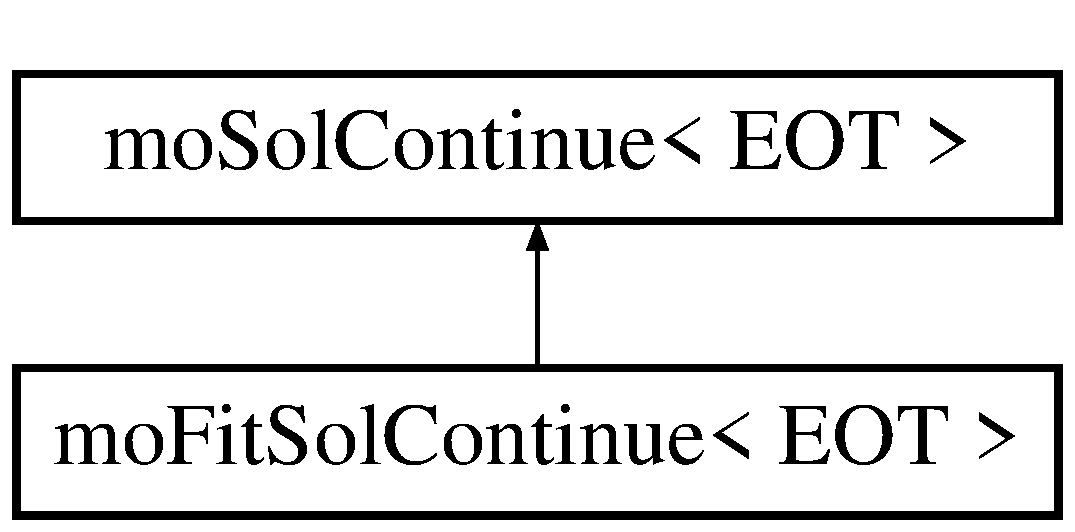
\includegraphics[height=4cm]{classmo_fit_sol_continue}
\end{center}
\end{figure}
\subsection*{Public Types}
\begin{CompactItemize}
\item 
typedef EOT::Fitness {\bf Fitness}\label{classmo_fit_sol_continue_369ed94a788d8bdc08d5554f7669376f}

\begin{CompactList}\small\item\em Alias for the fitness. \item\end{CompactList}\end{CompactItemize}
\subsection*{Public Member Functions}
\begin{CompactItemize}
\item 
{\bf moFitSolContinue} ({\bf Fitness} \_\-\_\-fitness, bool \_\-\_\-minimization=true)
\begin{CompactList}\small\item\em Basic constructor. \item\end{CompactList}\item 
bool {\bf operator()} (const EOT \&\_\-\_\-sol)
\begin{CompactList}\small\item\em Function that activates the stopping criterion. \item\end{CompactList}\item 
void {\bf init} ()\label{classmo_fit_sol_continue_670bd895b4edfcd3aebb40d2295d7f7c}

\begin{CompactList}\small\item\em Procedure which allows to initialise all the stuff needed. \item\end{CompactList}\end{CompactItemize}
\subsection*{Private Attributes}
\begin{CompactItemize}
\item 
{\bf Fitness} {\bf fitness}\label{classmo_fit_sol_continue_87d0ba8f2f76f61c89317eed5f094dfc}

\begin{CompactList}\small\item\em Fitness target. \item\end{CompactList}\item 
bool {\bf minimization}
\begin{CompactList}\small\item\em Flag that indicate if there is a minimization (true) or a maximization (false) of the fitness value. \item\end{CompactList}\end{CompactItemize}


\subsection{Detailed Description}
\subsubsection*{template$<$class EOT$>$ class moFitSolContinue$<$ EOT $>$}

One possible stop criterion for a solution-based heuristic. 

The stop criterion corresponds to a fitness threshold gained. 



Definition at line 21 of file moFitSolContinue.h.

\subsection{Constructor \& Destructor Documentation}
\index{moFitSolContinue@{moFitSolContinue}!moFitSolContinue@{moFitSolContinue}}
\index{moFitSolContinue@{moFitSolContinue}!moFitSolContinue@{moFitSolContinue}}
\subsubsection{\setlength{\rightskip}{0pt plus 5cm}template$<$class EOT$>$ {\bf moFitSolContinue}$<$ EOT $>$::{\bf moFitSolContinue} ({\bf Fitness} {\em \_\-\_\-fitness}, bool {\em \_\-\_\-minimization} = {\tt true})\hspace{0.3cm}{\tt  [inline]}}\label{classmo_fit_sol_continue_667090eca00b8532524f8e0a6e988fed}


Basic constructor. 

\begin{Desc}
\item[Parameters:]
\begin{description}
\item[{\em \_\-\_\-fitness}]The fitness to reach. \item[{\em \_\-\_\-minimization}]Indicate if the the aim is to maximize or minimize the fitness. \end{description}
\end{Desc}


Definition at line 34 of file moFitSolContinue.h.

\subsection{Member Function Documentation}
\index{moFitSolContinue@{moFitSolContinue}!operator()@{operator()}}
\index{operator()@{operator()}!moFitSolContinue@{moFitSolContinue}}
\subsubsection{\setlength{\rightskip}{0pt plus 5cm}template$<$class EOT$>$ bool {\bf moFitSolContinue}$<$ EOT $>$::operator() (const EOT \& {\em \_\-\_\-sol})\hspace{0.3cm}{\tt  [inline, virtual]}}\label{classmo_fit_sol_continue_fa9f0a15f99c998115cae9b456403a27}


Function that activates the stopping criterion. 

Indicates if the fitness threshold has not yet been reached.

\begin{Desc}
\item[Parameters:]
\begin{description}
\item[{\em \_\-\_\-sol}]the current solution. \end{description}
\end{Desc}
\begin{Desc}
\item[Returns:]true or false according to the value of the fitness. \end{Desc}


Implements {\bf eoUF$<$ const EOT \&, bool $>$}.

Definition at line 44 of file moFitSolContinue.h.

References moFitSolContinue$<$ EOT $>$::fitness, and moFitSolContinue$<$ EOT $>$::minimization.

\subsection{Member Data Documentation}
\index{moFitSolContinue@{moFitSolContinue}!minimization@{minimization}}
\index{minimization@{minimization}!moFitSolContinue@{moFitSolContinue}}
\subsubsection{\setlength{\rightskip}{0pt plus 5cm}template$<$class EOT$>$ bool {\bf moFitSolContinue}$<$ EOT $>$::{\bf minimization}\hspace{0.3cm}{\tt  [private]}}\label{classmo_fit_sol_continue_a4c90279f00774d9868a2e38ead45696}


Flag that indicate if there is a minimization (true) or a maximization (false) of the fitness value. 

It can be interesting to know this information because some solution-based metaheuristics can generate solution with a fitness that is worse that the best known fitness (in this case, the counter is not reinitialized). 

Definition at line 72 of file moFitSolContinue.h.

Referenced by moFitSolContinue$<$ EOT $>$::operator()().

The documentation for this class was generated from the following file:\begin{CompactItemize}
\item 
moFitSolContinue.h\end{CompactItemize}
